\item In the arrangement shown in Fig. 1.16 the bodies have masses \( m_0, m_1, m_2 \), the friction is absent, the masses of the pulleys and the threads are negligible. Find the acceleration of the body \( m_1 \). Look into possible cases.
    \begin{center}
        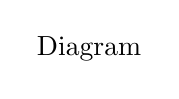
\begin{tikzpicture}
            \node at (0, 0) {Diagram};
        \end{tikzpicture}
    \end{center}
